\documentclass[a4paper,12pt]{article}
%%
\usepackage[english]{babel}
\usepackage[utf8x]{inputenc}
\usepackage{subfig}
%%
\usepackage{vmargin}
\setpapersize{A4}
\setmargnohfrb{2cm}{2cm}{2cm}{2cm}
\setlength{\parindent}{0mm}
%%
\usepackage{graphicx}
%%
\usepackage{amsmath}


\begin{document}
{\bf Monte Carlo Simulations -- spring 2018 \hfill Emil Levo\\ Final Project}\\
\\

\section{Introduction}

As the final project for this course, we were tasked with simulating a simple traffic jam. The system to be simulated is a set of discrete points that make up a one-dimensional road, where one point can be occupied by one, and only one car at a time. The cars can only move forward to empty points on the road and cannot surpass each other. The road is periodic, so that once a car moves while positioned at the end of the road it returns to the beginning of the road. The rate for a car to move one step forward is directly proportional to the empty road points in front of it until the next car. The cars should be moved randomly but with probabilites proportional to their moving rates and the average time increase should be physically correct over many MC steps.

For this purpose we have written a simple KMC code provided alongside with this report. We chose the KMC method since we are dealing with a system of discrete points that are moved based on their movement rates that can easily be gathered into a cumulative function. Then we can also naturally update the time of the system with a timestep $\Delta t = -\frac{\log u}{R} $ where $u$ is a random number between 0 and 1, and $R$ is the total rate of the system (final entry in the cumulative function). The simulated traffic jam is visualised as instructed in the project assignments, i.e. the road is printed at specific steps with an "X" representing a car and an empty space an empty point on the road. Additionally the time and step of the system is printed.

The following directories are included in the submitted file:

\begin{enumerate}
\item {\bf{src/}} : Contains the main code and all needed modules.
\item {\bf{run/}} : Contains the program excecutable once the code is compiled and some output data once the program is ran.
\item {\bf{report/}} : Contains the report pdf and everything needed to compile it.
\end{enumerate} 

Additionally the submitted file includes a {\bf{Makefile}} for compiling the code. For a succesful compilation of the code it should be enough to run the command {\bf{make}} in the project directory, and for cleaning the project directory use {\bf{make clean}}. The code should be compiled and the final excecutable named {\bf{jam}} moved to the {\bf{run/}} directory automatically. If for some reason the {\bf{Makefile}} should not work, one can also manually compile the code in the {\bf{src/}} directory and then move the executable to the run directory with the commands: \\

	{\bf{gfortran -c -O2 src/mer.f90 src/subs.f90 src/ana.f90 src/main.f90}} \\
	{\bf{gfortran -o jam mer.o subs.o ana.o main.o}} \\
	{\bf{mv jam run/}}

\newpage
\section{The Code}
The code itself is divided into one main code and three modules:

\begin{enumerate}
\item {\bf{main.f90}} : Contains main KMC loop.
\item {\bf{mer.f90}} : Contains Mersennes Twister RNG.
\item {\bf{subs.f90}} : Contains subroutines and functions for actual simulations.
\item {\bf{ana.f90}} : Contains subroutines and functions for analysis.

\end{enumerate}


To handle the road with the cars a specific type named "car" was created. The "car" type contains four things: A boolean for indicating if it is a car or an empty space, an id for the "car", the position of the "car" and the movement rate. The road is then handled as an array of "cars" (actual cars and empty spaces).

When initializing the simulation, cars are placed on even spaces on the road. If there are too many cars to be placed evenly, then the rest of the cars are placed in a queue in the beginning of the road. In the initialization and every step of the KMC algorithm the rates for the cars are calculated and the cumulative function updated. The car to be moved is chosen by generating a random number and then picking the corresponding car in the cumulative function.

During the simulation the state of the road is printed with the time and MC-step at a chosen interval. An "X" specifies a car and an empty space " " is an empty space on the road. An example can be found in Fig.~\ref{pic:ex}

\begin{figure}[h]
\centering
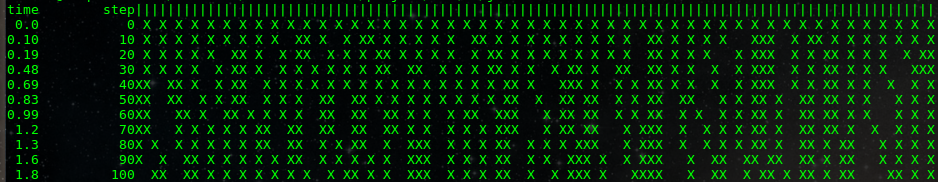
\includegraphics[width=\columnwidth]{road1.png}
\caption{Example print of a traffic jam simulation (50 cars, 100 spaces).}
\label{pic:ex}
\end{figure}

When the code is succesfully compiled, it can be ran in the {\bf{run/}} directory. Running the program needs a total of seven commmand line arguments for a succesful execution. The arguments are (given in the following order):

\begin{enumerate}
\item An integer seed for the RNG.
\item Number of cars $N$.
\item Length of road $L$.
\item Number of simulation steps.
\item The interval at which the road is to be printed to the screen.
\item Traffic camera on/off with integer 1/0.
\item Speed limit on/off with integer 1/0.
\end{enumerate} 

The program will not run unless all arguments are there. After a succesful run, there should be a file named {\bf{dat.out}} in the {\bf{run/}} directory. The output file contains columns with the time, step, number of queues and mean length of queues in the simulation step.

\section{Results}
\begin{enumerate}
\item

For the first problem in the project we were to simulate cars spaced evenly on every second place on the road, i.e. $N/L=0.5$. Then we ran the simulation from some thousand steps to some million steps. An example simulation can be seen in Fig.~\ref{pic:road1} with every 20th step printed to the screen. From the figure it can be clearly seen that the queues are moving to the left, which makes sense since a car can only join a queue from the left and leave it to the right.

\begin{figure}[h]
\centering
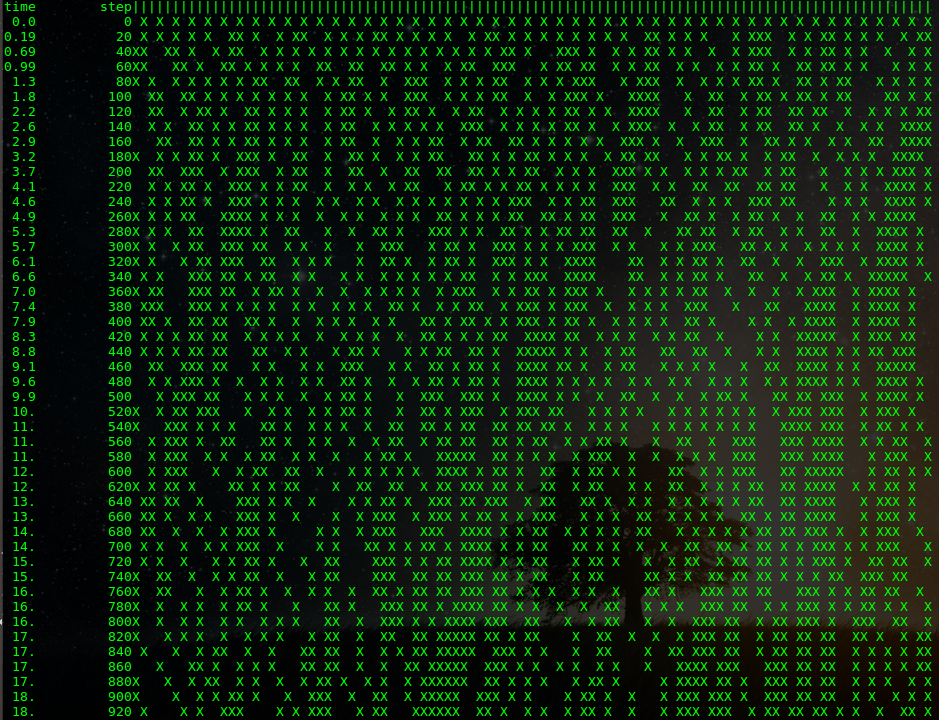
\includegraphics[width=\columnwidth]{road2.png}
\caption{Example simulation with $N=50$ and $L=100$.}
\label{pic:road1}
\end{figure}

This exact simulation presented in Fig.~\ref{pic:road1} should be achieved by running the {\bf{jam}} executable with the command

{\bf{./jam 1425234 50 100 1000 20 0 0}}

For estimating the velocity of the queue propagation can be done visually from the screen print. If an appropriate interval for printing is chosen, the queues movement can be seen more clearly. The simulation seen in Fig.~\ref{pic:vel} can be produced by running the program with

{\bf{./jam 1425234 50 100 100000 50 0 0}} 

Then let us inspect the distance travelled of one queue in the system. Some lines are drawn into the figure for better visualisation of the distance travelled and the timelapse. The chosen queue moves approximately 61 blocks during the time $\Delta t = 49.0 - 1.8 = 47.2 $. In this case the queue in question would have a propagation velocity (in our simulation units of length and time) of $ v = 61/47.2 \approx 1.29 $.

\begin{figure}[h]
\centering
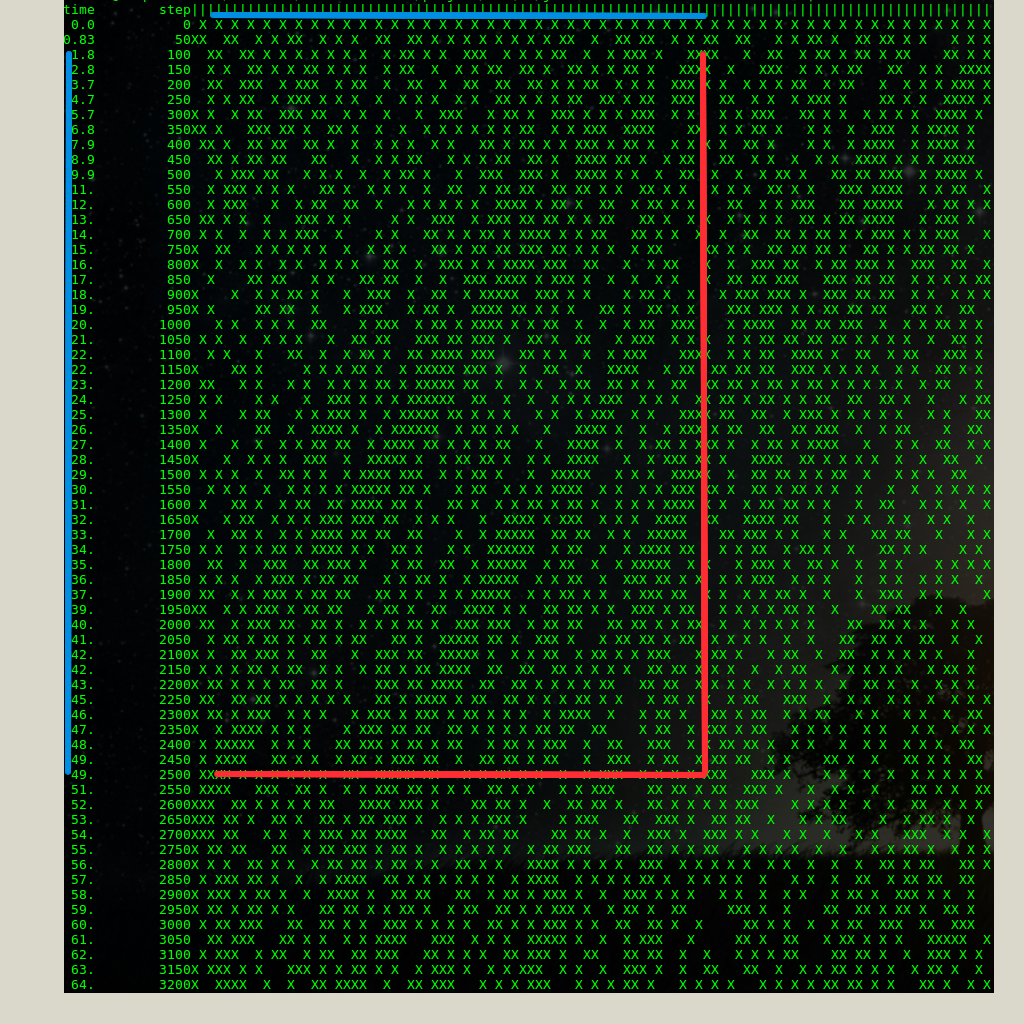
\includegraphics[width=\columnwidth]{vel.png}
\caption{}
\label{pic:vel}
\end{figure}

We ran three additional simulations for the velocity investigation resulting in the data presented in Tab.~\ref{tab:vel}.

\begin{table}[h!]
\centering
\begin{tabular}{|c|c|c|}
\hline
Steps & $\Delta t$ & $v$ \\ \hline
61 & 47.2 & 1.29 \\ \hline
28 & 26.09 & 1.07 \\ \hline
29 & 25.9 & 1.12 \\ \hline
29 & 20.0 & 0.97 \\ \hline
\end{tabular}
\caption{Table for velocity data.}
\label{tab:vel}
\end{table}

From this data we can get a mean of $ \overline{v} = 1.11 \pm 0.12 $ which is a very crude result but adequate for a mere estimation of the queue propagation velocity.

\newpage
\item

For the second problem we wanted to investigate the number and length of queues with varying car density. We ran nine different car densities $N/L = 0.1,0.2,...,0.9$ on a road with length $L=100$. Each simulation was ran a hundred times with a different seed every time (the seeds were 1,2,...,100). All simulations were ran with 10000 MC-steps of which all were printed to the {\bf{dat.out}} files and the last 5000 were analysed. The reason for this amount of steps was so that the system would surely be equilibrated before the analysis.

For the analysis in this problem we calculated the mean of both length and number of queues for the simulation and the corresponding errors. The analysis script {\bf{ana.sh}} used can be found in the {\bf{run/}} directory. The resulting figures from the data can be seen in Fig.~\ref{pic:prob2}.

\begin{figure}[h]
\centering
\subfloat[Length of queues plotted against number of cars.]{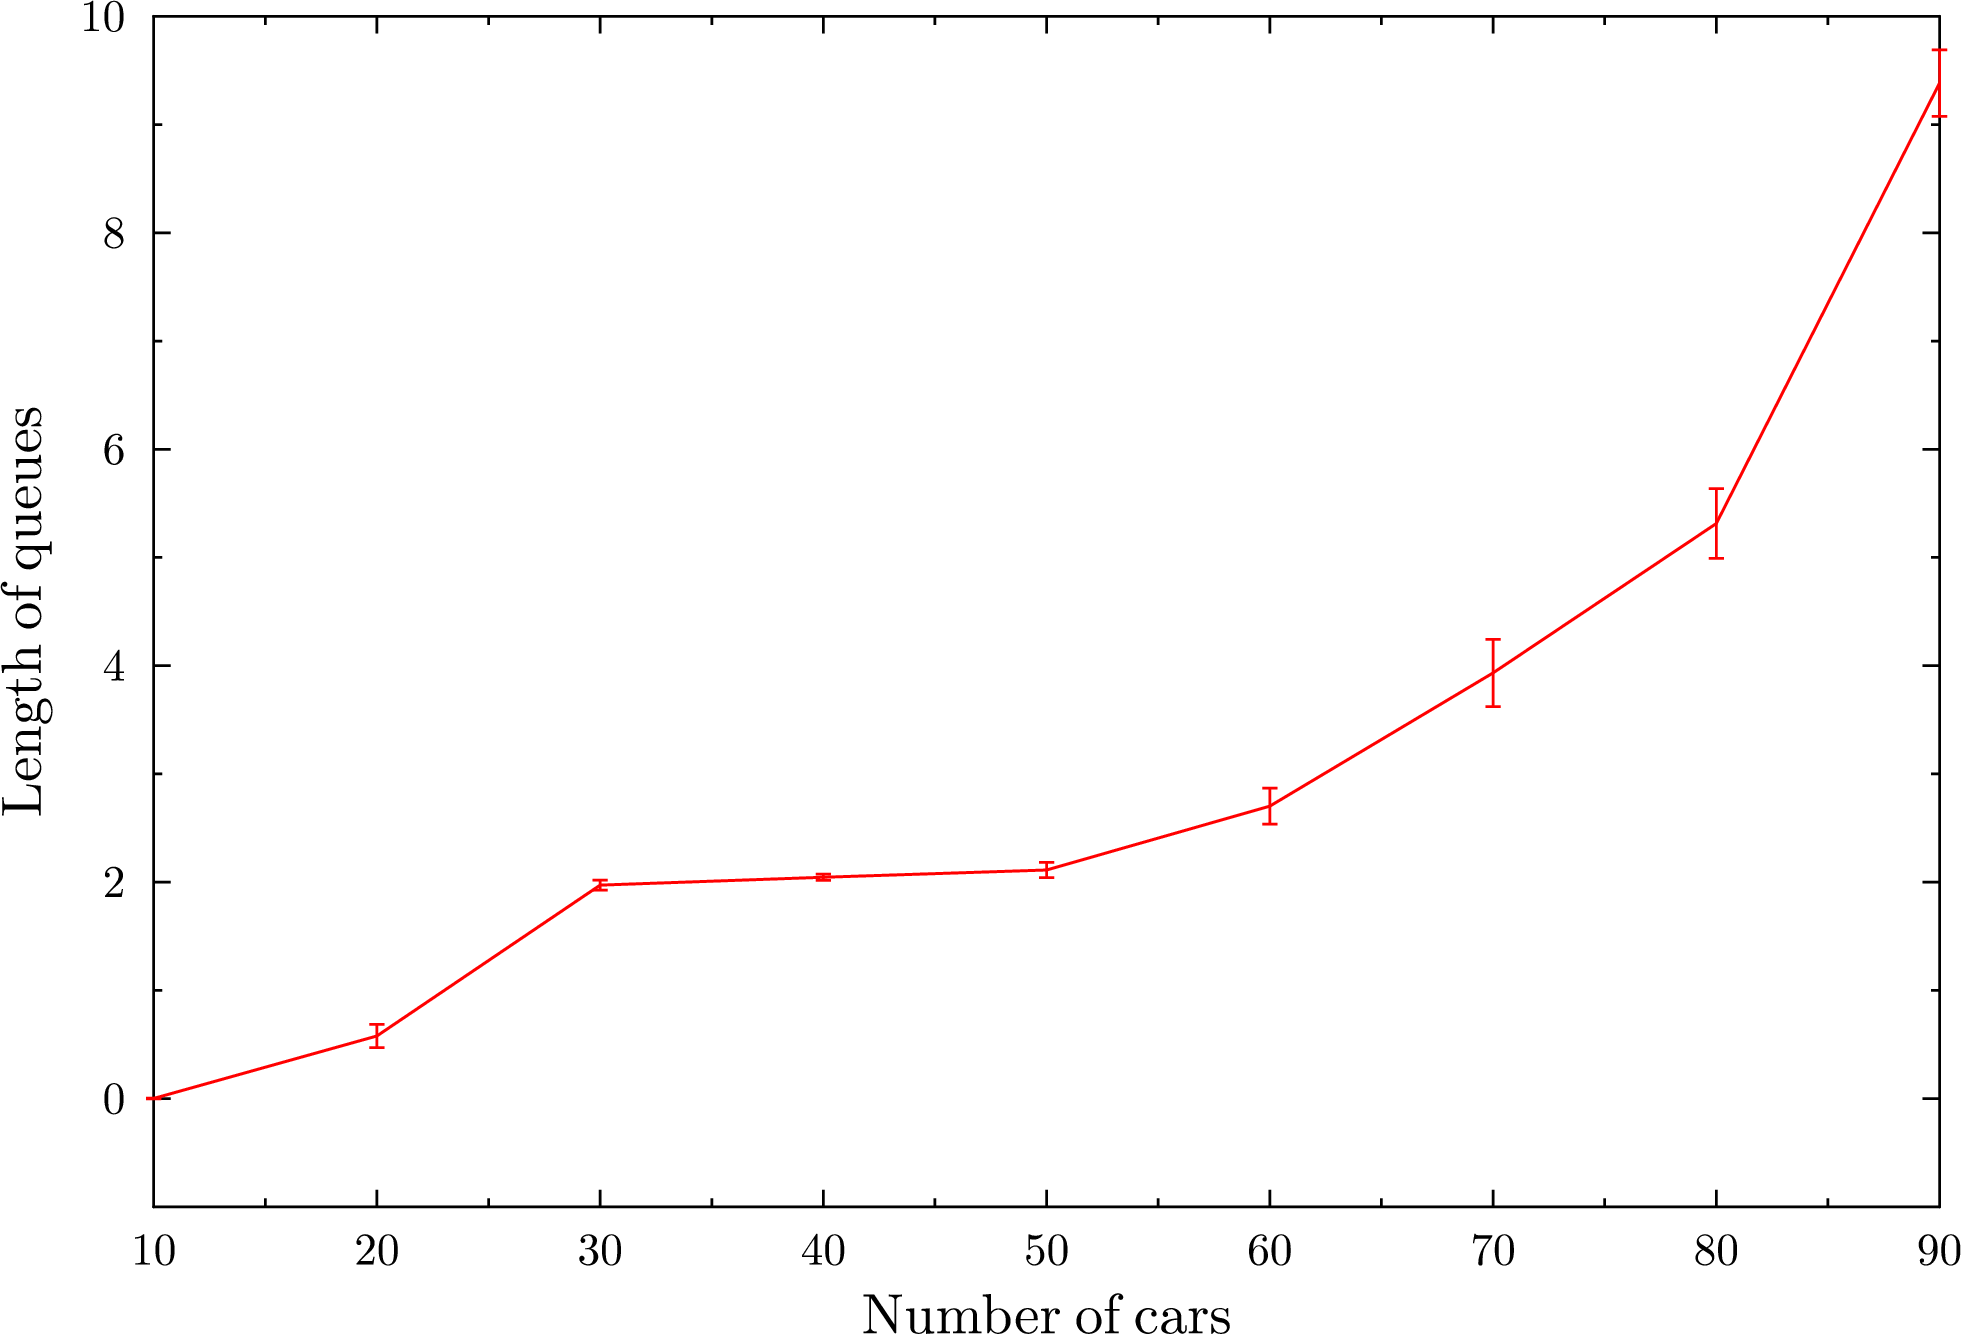
\includegraphics[width=0.5\columnwidth]{queuelen.png}}
\subfloat[Number of queues plotted against number of cars.]{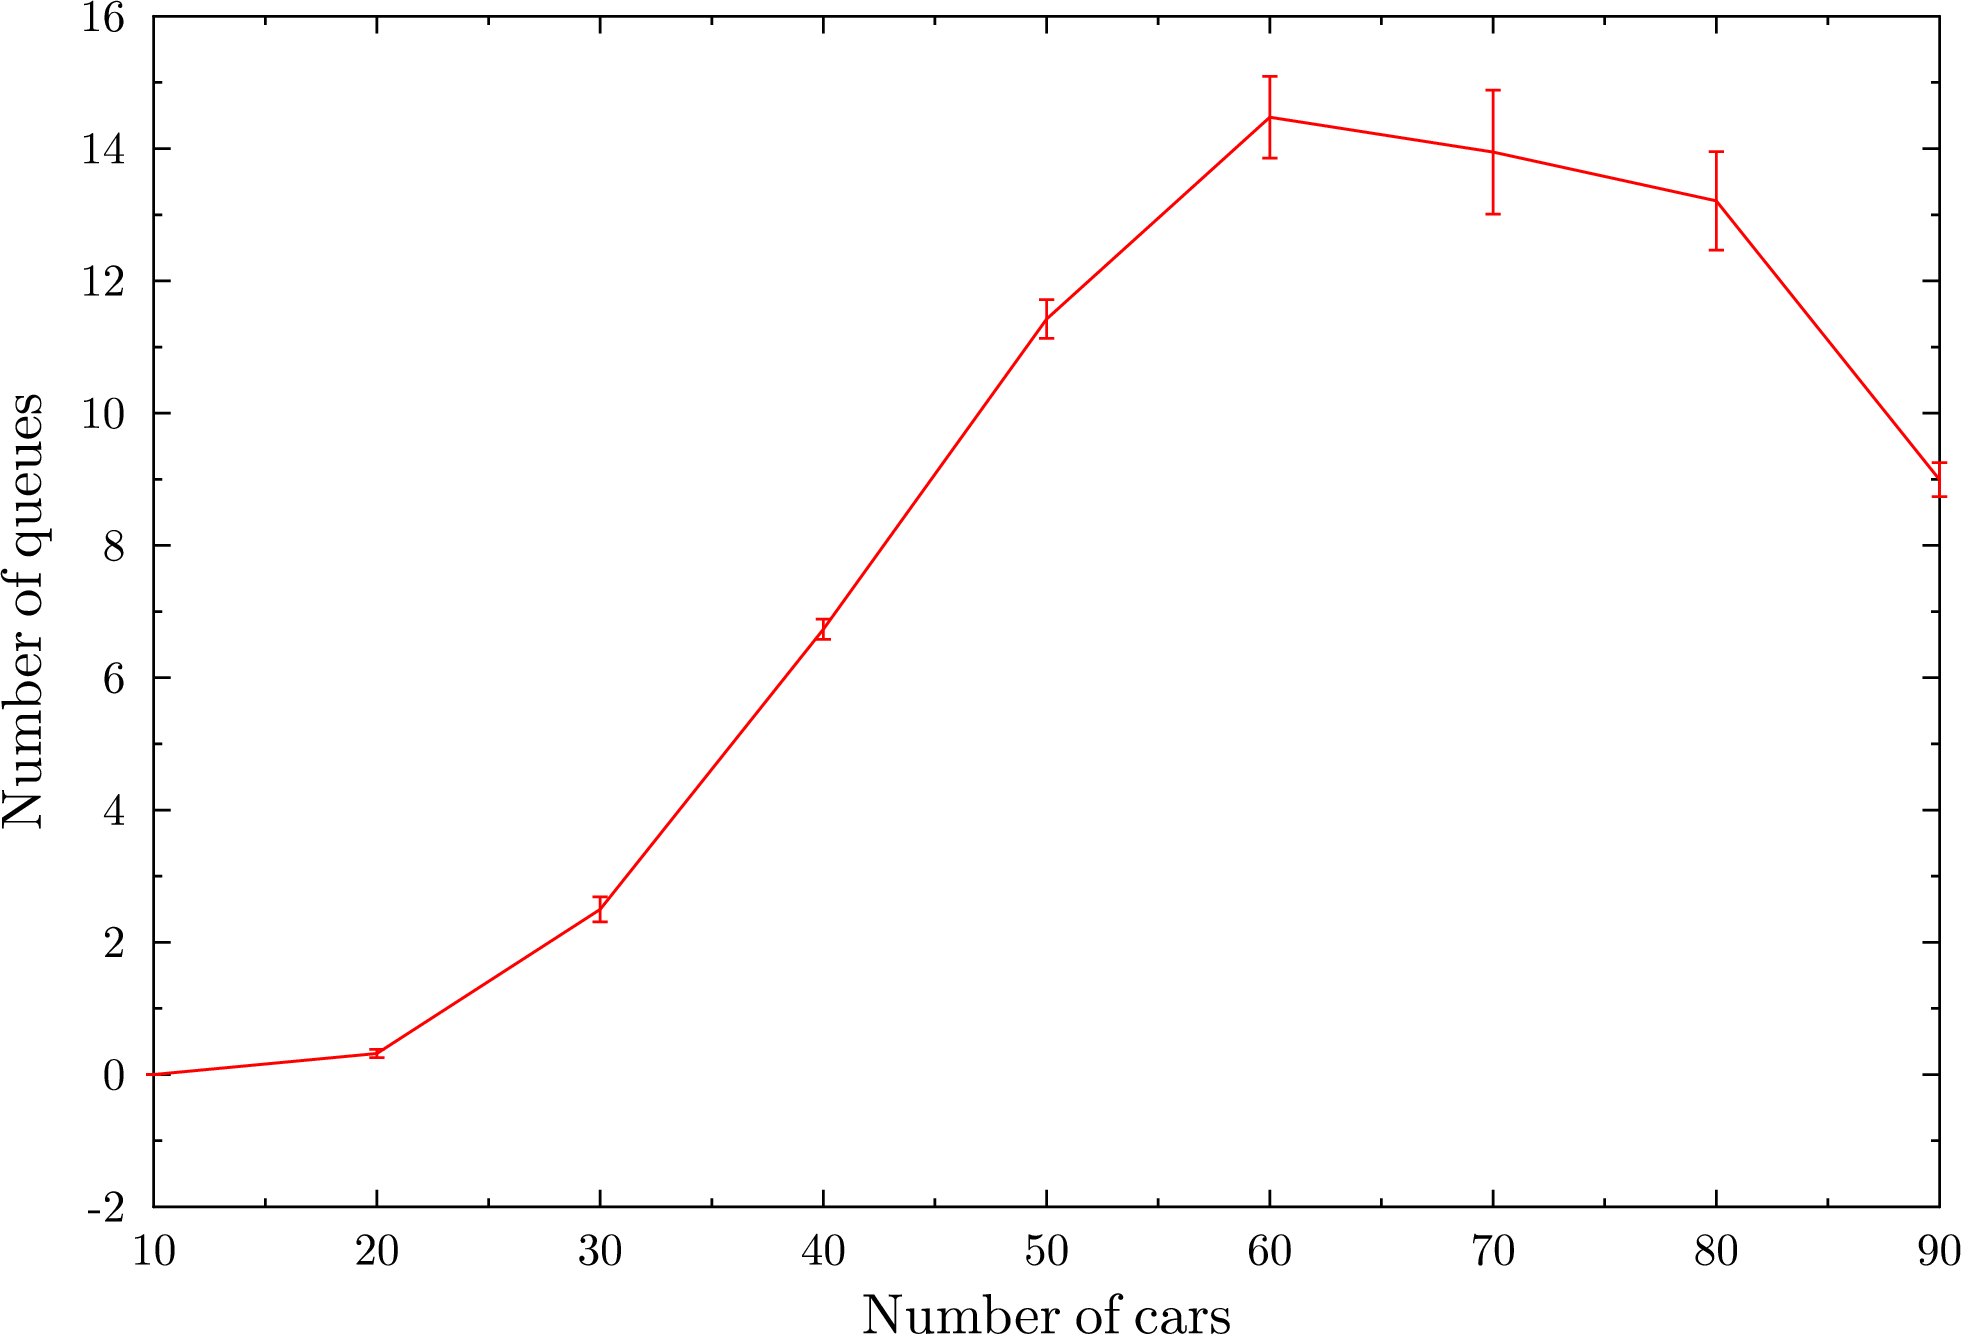
\includegraphics[width=0.5\columnwidth]{queuenum.png}}
\caption{The resulting graphs for problem 2.}
\label{pic:prob2}
\end{figure}

In Fig.~\ref{pic:prob2} a) we can see an almost exponential growth of the length of the queues which makes sense, since we are filling up the empty spaces on the road. In Fig.~\ref{pic:prob2} b) we can see in the beginning somehing of a parabolic growth that starts plateauing after $N/L=0.5$ and decreasing after $N/L=0.7$. This makes sense since we are creating more of a traffic jam with the increasing density, until we have filled up the road too much so that there is room only for a smaller number of queues of greater length. Eventually when the road is filled enough there will be only one queue with the length $99$ (with a hundred cars the jam cannot move). We can also conclude that there is no significant amount of cars on the road below $N/L=0.3$.

To obtain these exact results, run the bash script {\bf{start.sh}} in the {\bf{run/}} directory and analyse the resulting data with {\bf{ana.sh}}. The output should look like the data found in the file {\bf{queue.dat}} in the {\bf{run/}} directory. There is a gle file {\bf{plotR.gle}} for plotting of the output data.

\newpage
\item
For the third proble we inserted a traffic cam halfway on the road. This would essentially mean that a car would slow down because of the cam and then create a queue because of it. Now remember, to run a simulation with a traffic cam, one needs to activate it by turning the sixth argument to 1 like so:

{\bf{./jam 13564 20 100 100000 10 1 0}}

Running the program with this command will produce what can be seen in Fig.~\ref{pic:cam}

\begin{figure}[h]
\centering
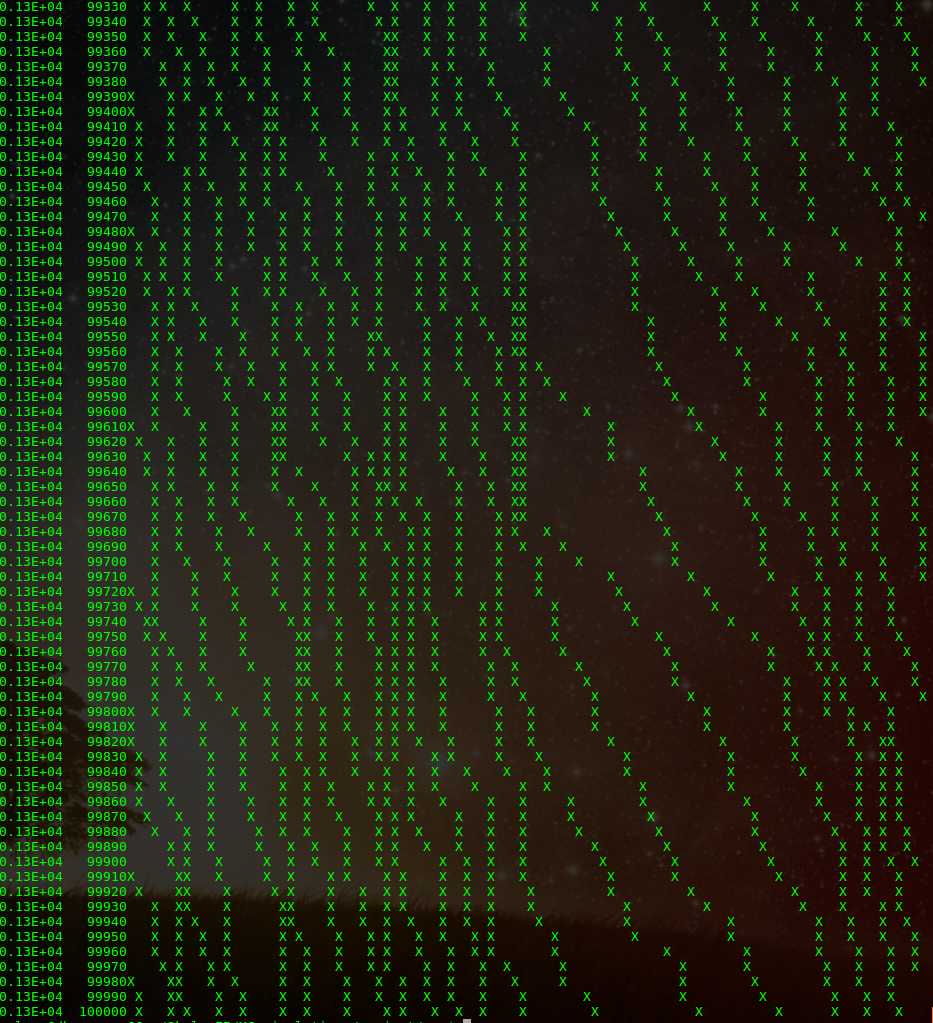
\includegraphics[width=\columnwidth]{trafcam.png}
\caption{Simulation with traffic camera.}
\label{pic:cam}
\end{figure}

As we can see there is a staggering in the middle of the road (where the camera is). A car at the camera will slow down and speed up again once it is past it. We ran the exact same simulation as in the previous problem and compared the resulting data with Fig.~\ref{pic:prob2} b). In the figure we can see a slight increase in the number of queues in the beginning of the simulations. This is an indication towards a higher possibility of queue formation at lower densities. So the answer is yes, the camera can produce queues at low densities that otherwise would not produce queues. There is also a greater error in the mean, meaning that there is a bigger spread int the number of queues data. 

To obtain these exact results, run the bash script {\bf{start.sh}} in the {\bf{run/}} directory and analyse the resulting data with {\bf{ana.sh}}. The output should look like the data found in the file {\bf{cam.dat}} in the {\bf{run/}} directory.

\begin{figure}[h]
\centering
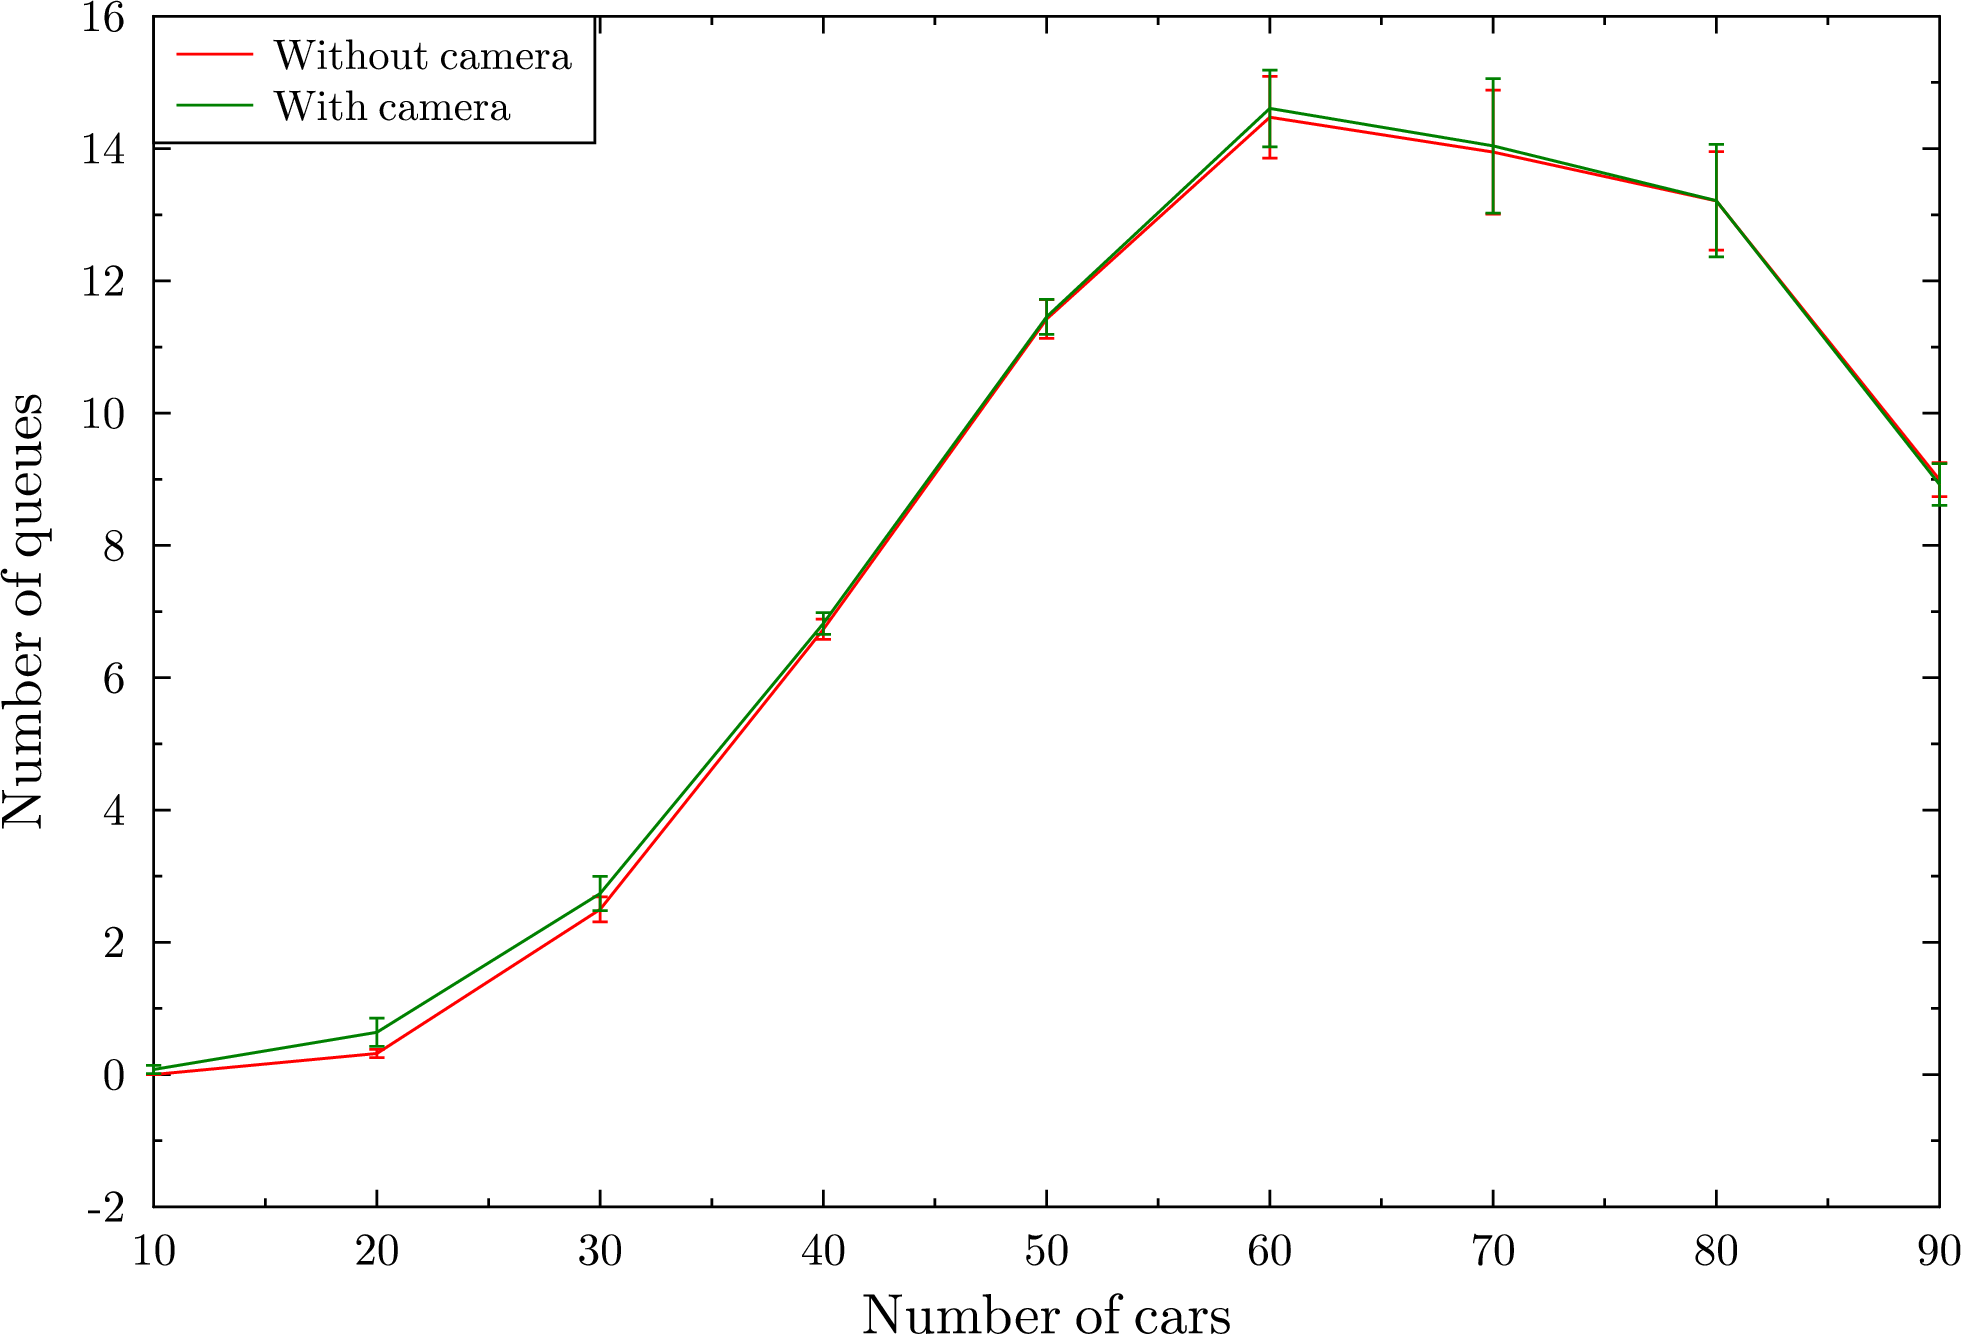
\includegraphics[width=0.7\columnwidth]{cam.png}
\caption{Number of queue comparison between simulations with and without traffic camera.}
\end{figure}

\item
For the final problem we set a speed limit on all cars in the system. The way we did this, was simply by reducing a cars rate to three even if there were more than three empty spaces in front of it. Again one needs to remember to activate the speed limit. This time change the seventh command line argument to 1, like so:

{\bf{./jam 13564 50 100 100000 20 0 1}}

The resulting screen with this command can be seen in Fig.\ref{pic:limit}. From the figure it is clear that the queues are still moving to the left. It would be nonsensical for the queues to move to the right, since new cars still join the queues from the left.

We ran again the exact same simulation as in problems 2, but with the speed limit activated. The resulting data comparison between the simulations with and without the limit can be seen in Fig.~\ref{pic:speedlimit}. As we can see, the two plots coincide pretty much perfectly so the answer is no, the speed limit will not cause queues at low densities, just like in the original case.

To obtain these exact results, run the bash script {\bf{start.sh}} in the {\bf{run/}} directory and analyse the resulting data with {\bf{ana.sh}}. The output should look like the data found in the file {\bf{limit.dat}} in the {\bf{run/}} directory.

\begin{figure}[h]
\centering
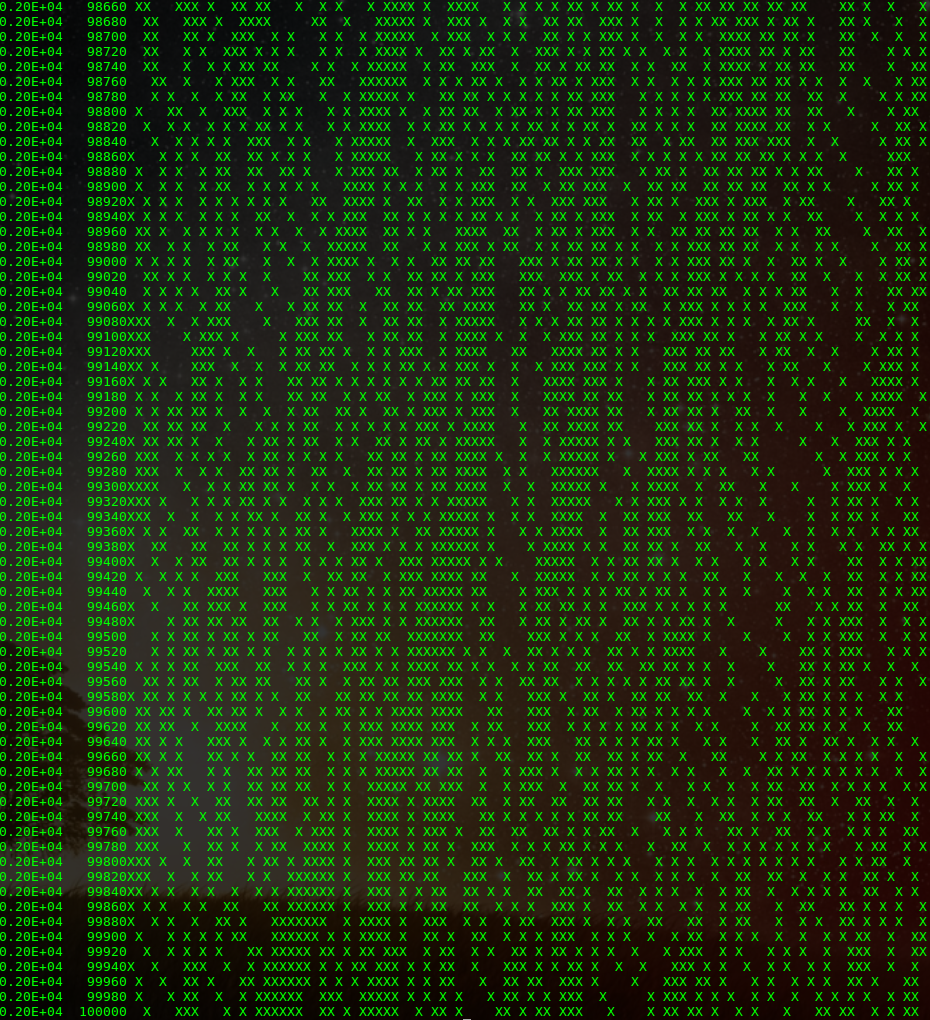
\includegraphics[width=\columnwidth]{limit.png}
\caption{Simulation with speed limit.}
\label{pic:limit}
\end{figure}

\begin{figure}[h]
\centering
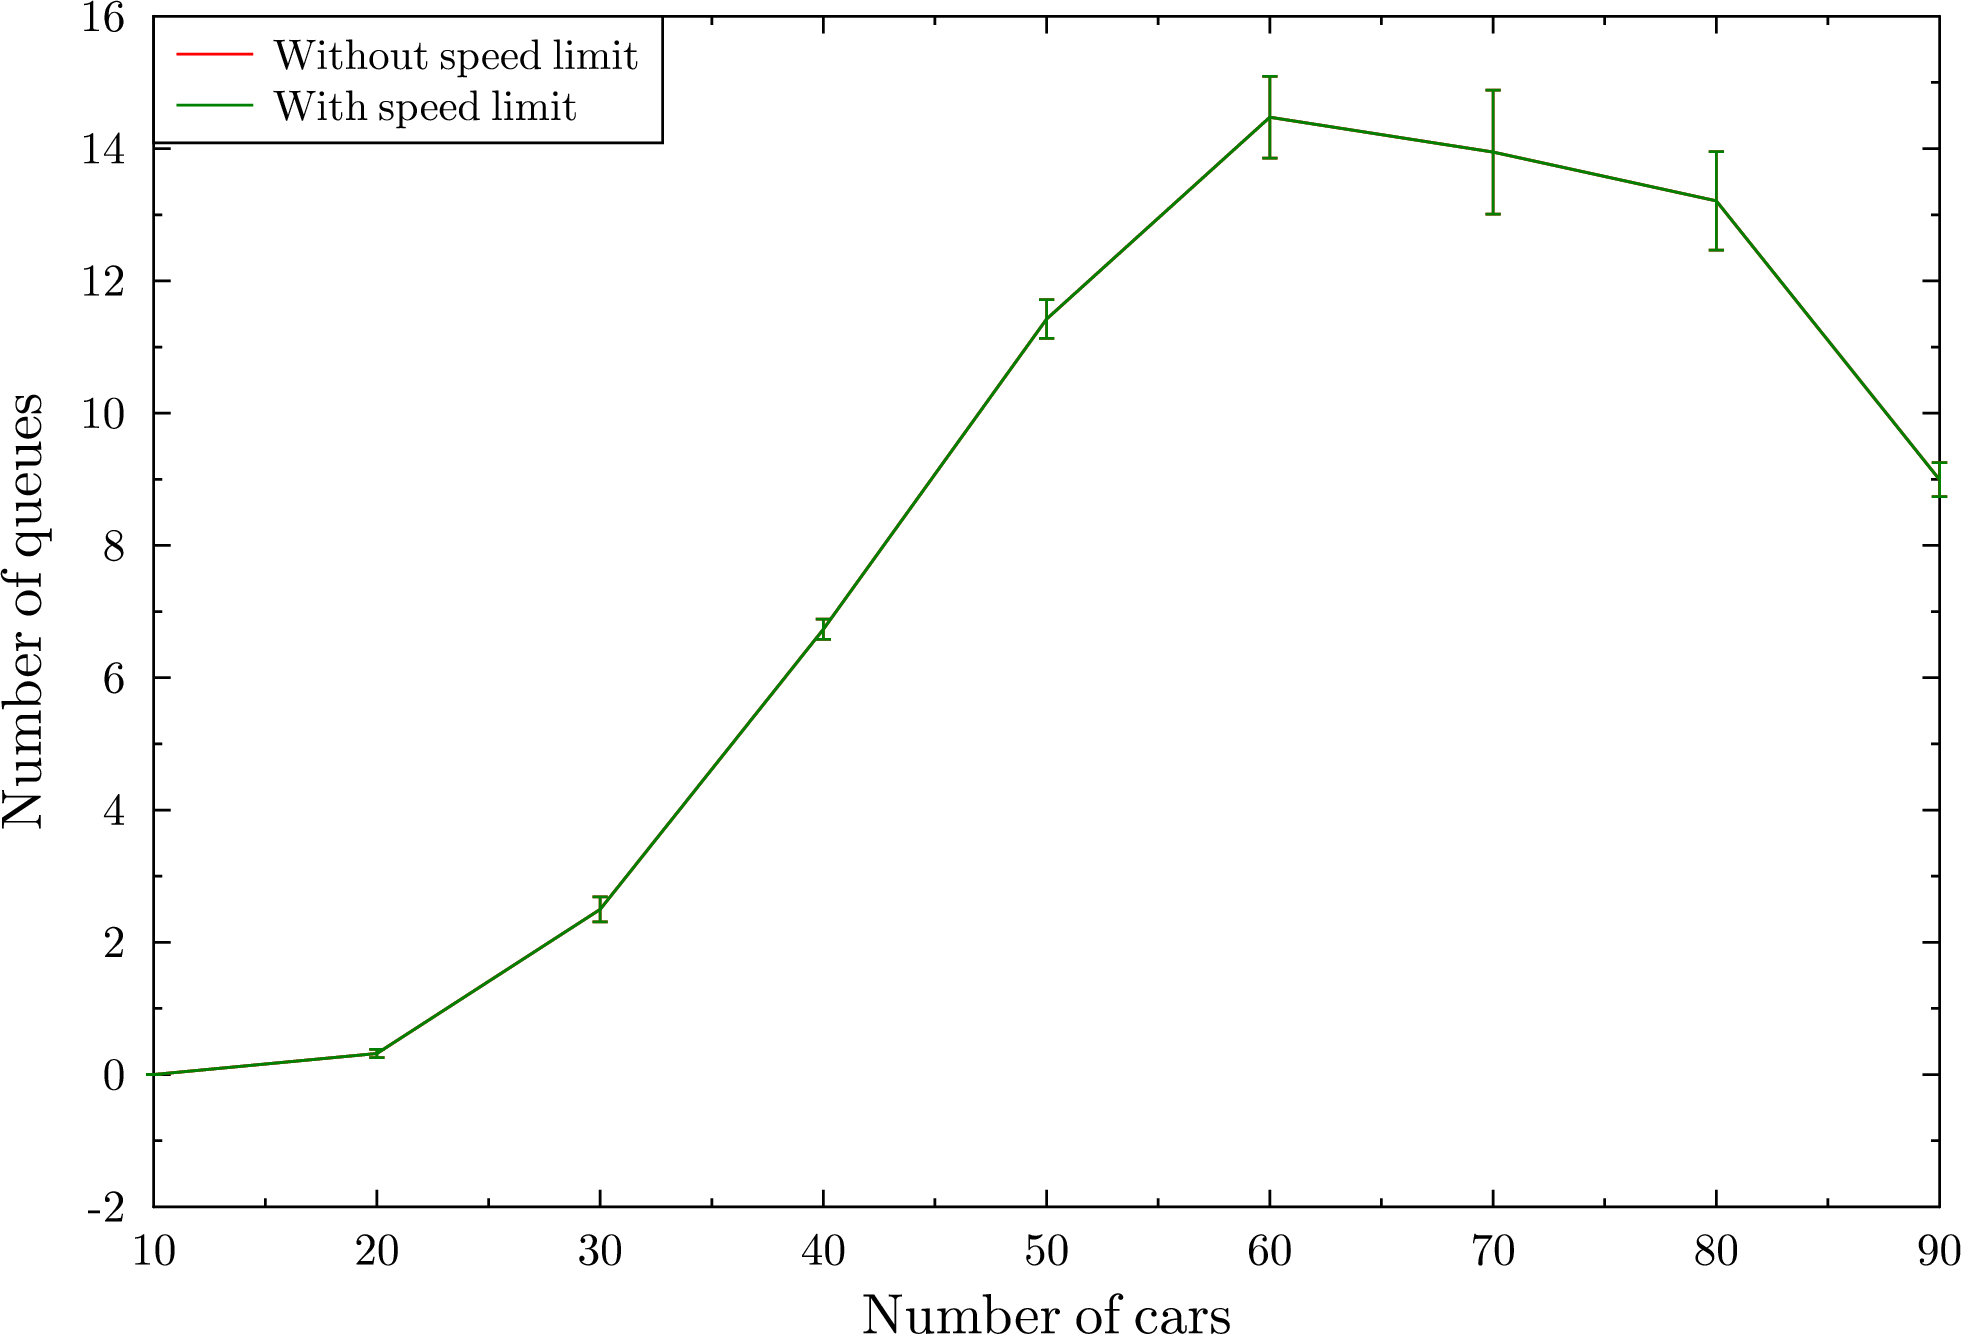
\includegraphics[width=0.7\columnwidth]{speedlim.png}
\caption{Comparison between simulation with and without speed limit.}
\label{pic:speedlimit}
\end{figure}

\end{enumerate}


\end{document}
